\documentclass[runningheads]{llncs}
\usepackage[newfloat]{minted}
\setminted[cpp]{
frame=lines,
linenos,
breaklines,
fontsize=\footnotesize,
framesep=2mm
}
\usepackage{caption}
\usepackage{graphicx}
\usepackage[portuguese]{babel}
\usepackage{hyphenat}
\usepackage{lscape}
\usepackage{microtype} % melhora a formatação do texto para evitar overfull box, entre outros
\usepackage{hyperref}
% to insert sourcecode
\newenvironment{code}{\captionsetup{type=listing}}{}
\SetupFloatingEnvironment{listing}{name=\underline{\textbf{CGDraw} Source Code}}

\begin{document}
%
\title{Relatório Computação Grafica - Fase 2}
\author{Marco Sousa\inst{1,2}\orcidID{62608} \and
    José Malheiro\inst{1,2}\orcidID{93271} \and
    Miguel Fernandes\inst{1,2}\orcidID{94269}}
%
\institute{Universidade do Minho\\
    \and Licenciatura em Engenharia Informática, Braga, Portugal}
%
\maketitle              % typeset the header of the contribution
%
\begin{abstract}
    Devido à influência crescente de novas indústrias, nomeadamente a de jogos e cinematográfica, a integração dos meios para gerar graficamente novos ambientes é da mais elevada importância.
    No âmbito de um primeiro contacto esta vasta área, de computação gráfica, será apresentada a conceção da primeira fase do projeto académico realizado pelo grupo.
    Este relatório engloba a conceção de duas aplicações, para gerar e apresentar figuras geométricas, a partir de valores dados.
    \keywords{ OpenGL \and GLUT \and Figuras Geométricas \and 3D \and C++}
\end{abstract}

\section{Introdução}

\subsection{Contextualização}

No seguimento da fase I do projeto da disciplina de \textit{Compucação Gráfica} da Licenciatura em
Engenharia Informática da Universidade do Minho, foi proposto a aplicação de transformações geométricas
ao motor previamente desenvolvido, assim como o desenvolvimento de um modelo sistema solar.

\subsection{Breve Descrição do Enunciado Proposto}
O principal foco da fase a que este relatório se remete é a aplicação de um conjunto de transformações geométricas,
tais como translação, rotação e escala de forma hierárquica a um conjunto de modelos.
Assim, a estrutura dos modelos é efetuada através da definição de grupos e respetivos subgrupos,
conforme exposto no enunciado.

Os grupos \textit{filhos} deverão adquirir as transformações geométricas dos \textit{pais},
i.e. as transformações são aplicados a todos os modelos e subgrupos.
As transformações geométricas devem ser aplicadas na mesma ordem que são definidas no ficheiro de \textit{input}.

Por último, foi proposto o desenvolvimento de um modelo \textbf{estático} do sistema solar, incluíndo o sol,
planetas e luas definidas de forma hierárquica.

\section{Trabalho Realizado}
Funcionalidades implementadas:
\begin{enumerate}
    \item Transformações geométricas aplicadas de forma hierárquica (\ref{sec:transf_geometricas})
          \begin{enumerate}
              \item Possibilidade de aplicar múltiplas vezes a mesma transformação
              \item Garantia de aplicação das transformações pela mesma ordem que a definida no ficheiro de \textit{input}
          \end{enumerate}
    \item Navegação com câmera $FPS$ (\ref{sec:camera_fps})
          \begin{enumerate}
              \item Acréscimo de escala de navegação
          \end{enumerate}
    \item Construção de modelo do sistema solar (\ref{sec:modelo_ss})
\end{enumerate}

\subsection{Transformações Geométricas} \label{sec:transf_geometricas}
Como consequência da arquitetura definida na fase $I$, a implementação desta fase foi facilitada.
Em particular, para aplicar as transformações geométricas de forma hierárquica, optou-se
por criar uma nova \mintinline{cpp}{class Transform} que se pode encontrar ao nível da
\mintinline{cpp}{class Group}.
Ao implementar desta forma, permitiu que um conjunto de transformações fosse aplicada em todo
o \textit{scope} do \textbf{Grupo} (seja modelos ou subgrupos).
Assim, pode-se encontrar a $Transform$ ao nível do objeto Group:

\begin{code}
    \captionof{listing}{Group}
    \label{code:group_h}
    \inputminted[firstline=12, lastline=18]{cpp}{../../Group.h}
\end{code}

Nesta classe ($Transform$), a primeira abordagem apenas permitia que se tivesse uma transformação
de cada tipo, sendo estas aplicadas pela ordem: translação, rotação e escala.
Após uma análise mais detalhada do enunciado e mediante as dificuldades encontradas
na construção do modelo do \textit{sistema solar}, verificou-se que seria necessário
a \textit{\textbf{engine}} ser capaz de aplicar múltiplas transformações do mesmo tipo,
no mesmo conjunto de elementos e que a sua ordem de aplicação poderia ser diferente daquela
definida de forma estática.
Assim, procedeu-se à alteração da \mintinline{cpp}{class Transform} para albergar um
\mintinline{cpp}{std::vector<transformation>}.

\begin{code}
    \captionof{listing}{Transformation}
    \label{code:struct_transformation}
    \inputminted[firstline=17, lastline=21]{cpp}{../../Transform.h}
\end{code}

Em termos concretos, pode-se encontrar a estratégia utilizada
representada no seguinte diagrama de sequência na figura \ref{fig:seq_transf_geom}.
Em suma, consiste em chamar de forma recursiva o método \mintinline{cpp}{void draw()} ao longo
da hierarquia do Grupo, Modelo e Subgrupos.

\subsection{Câmera $FPS$} \label{sec:camera_fps}
Optou-se por implementar a câmera do tipo $FPS$.
A sua implementação consistiu em utilizar uma biblioteca ("cartesian") desenvolvida pelo grupo para facilitar os cálculos
sobre pontos $3D$.

Durante o \textit{parsing} do ficheiro $XML$:
\begin{enumerate}
    \item \mintinline{cpp}{set_camera_pos(X, Y, Z)} - define a posição onde a câmera se encontra,
    a partir do elemento \mintinline{xml}{<position x="X" y="Y" z="Z" />}
    \item \mintinline{cpp}{set_camera_lookat(X, Y, Z)} - define a direção da câmera,
    a partir do elemento \mintinline{xml}{<lookAt x="X" y="Y" z="Z" />}
    \begin{enumerate}
        \item Cria-se um vetor entre os pontos $lookat$ e $position$
        \item Efetua-se a normalizalização do vetor para que seja unitário
        \item Armazena-se em duas estruturas distintas o valor em cartesiano e em polar
        (este último) permite posteriormente oscilar os ângulos $\alpha$ e $\beta$ para movimentar a câmera.
    \end{enumerate}
    \item \mintinline{cpp}{set_camera_up(X,Y,Z)} - define a orientação do vetor vertical da câmera a partir do 
    elemento \mintinline{xml}{<up x="X" y="Y" z="Z" />}
\end{enumerate}

Após efetuar o \textit{parsing} do xml, tem-se o estado inicial de navegação.
A partir deste, foi utilizado os métodos \mintinline{cpp}{move_camera(CAMenum t)} e
\mintinline{cpp}{move_lookat(double alpha, double beta)}.

A movimentação do $lookat$ consiste em incrementar o valor do $\alpha$ conforme o movimento do 
rato ao longo da janela.
Quanto ao primeiro - move_camera(CAMenum) efetua um movimento para a frente, trás, direita e esquerda.
Em qualquer um dos casos, é utilizado o vetor $lookat$ multiplicado por um escalar para movimentar a posição da câmera.
No caso de movimentar para a esquerda e direita, como a referência é para onde a câmera está a olhar,
utilizou-se uma rotação de [+-] 90$\deg$ e, posteriormente, movimentou-se a câmera.
Ao utilizar o vetor $lookAt$ garante-se que o movimento é uniforme e congruente com a sua dieração.

\subsection{Modelo do Sistema Solar} \label{sec:modelo_ss}
OK - Aplicação transformações geométricas
OK -- criação de vetor transformações no objeto Grupo (desta forma é aplicado a todos os seus elementos: modelos ou subgrupos)
OK --- aplica multiplas transformações por ordem definida (pode aplicar uma ou mais vezes a mesma transformação)
- Câmera FPS
-- implementação de escala para movmientação da câmera (botões + e - para aumentar ou reduzir a escala de movimento, respetivamente)

\begin{landscape}
    \begin{figure}
        \centering
        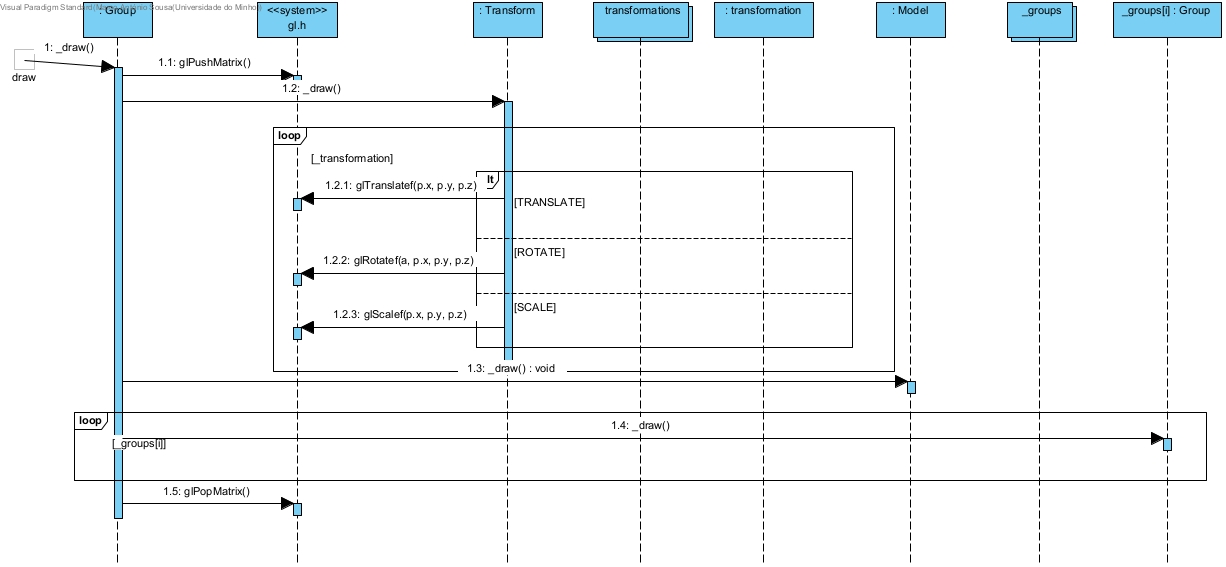
\includegraphics[width=\linewidth]{assets/geom_transf.jpg}
        \caption{Diagrama de sequência das transformações geométricas} \label{fig:seq_transf_geom}
    \end{figure}
\end{landscape}

\begin{landscape}
    \begin{figure}
        \centering
        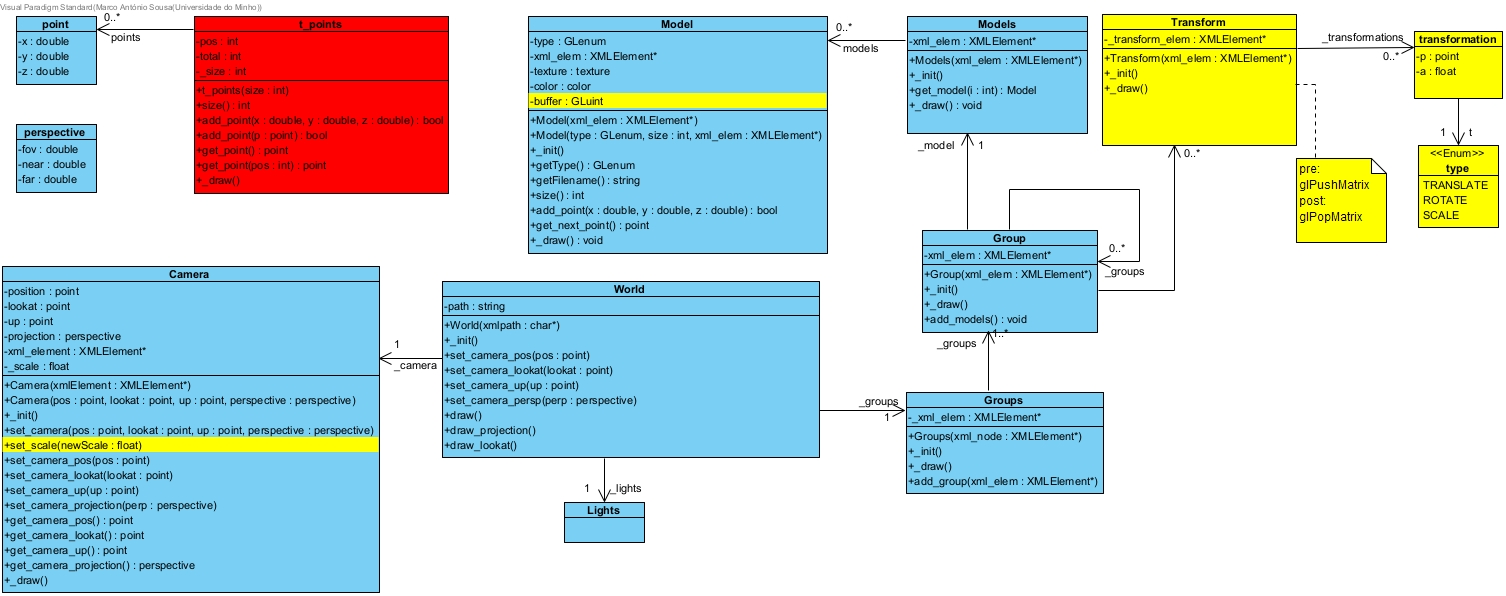
\includegraphics[width=\linewidth]{assets/world.jpg}
        \caption{Arquitetura da Aplicação - \textit{Alterações em relação à fase 1 a amarelo}.}
    \end{figure}
\end{landscape}



\section{Conclusão}
No contexto de um primeiro contacto com o ambiente gráfico inerente à cadeira, várias dificuldades surgiram na conceção da primeira fase do projeto.
A construção de objetos, com uma abstração ao plano \textbf{3D}, aliada à nomenclatura de uma nova linguagem, colocou questões sobre como atingir os resultados requiridos, em duas aplicações bem construídas dignas do nível académico do grupo.

Munidos com o auxílio da equipa docente, foi possível realizar a dinâmica proposta, o \textbf{generator} e a \textbf{engine}, com uma arquitetura multifacetada, tendo em consideração as futuras alterações das próximas fases do projeto.

Assim, o grupo apresenta uma solução que responde ao requisitos da fase inicial, procurando trazer outros elementos, como a adição da escolha da construção de um cilindro, como lecionado nas aulas práticas.

%
% ---- Bibliography ----
%
% BibTeX users should specify bibliography style 'splncs04'.
% References will then be sorted and formatted in the correct style.
%
% \bibliographystyle{splncs04}
% \bibliography{mybibliography}
%

\end{document}